\documentclass{beamer}
\usepackage[utf8]{inputenc}
\usepackage{graphicx}
\usetheme{default}
\usecolortheme{default}
\usepackage{enumitem}

\title[S10]{Section 9 : Gestion de portefeuille obligataire \\ $(2^{e}$ partie)}
\subtitle{GSF-3100 Marché des capitaux}
\author[SP. Boucher]{Simon-Pierre Boucher\inst{1}}
\institute[Université Laval]
{
  \inst{1}%
  Département de finance, assurance et immobilier\\
  Faculté des sciences de l'administration\\
  Université Laval}
\date[Automne 2021]{Automne 2021}

\begin{document}

\begin{frame}
  \titlepage
\end{frame}



\section{Analyse Moyenne-Variance}

\begin{frame}{Analyse Moyenne-Variance}
\begin{itemize}[label=\bullet]
\item La théorie du portefeuille telle que formulée par Harry Markowitz au début des années 1950 fournit des conseils pour la construction de portefeuilles.
\item Indique que trois paramètres sont importants dans la sélection des titres à incorporer dans un portefeuille.
\begin{enumerate}[label=\arabic*)]
\item La valeur moyenne attendue du rendement d'un actif 
\item La variance du rendement d’un actif
\item La covariance qui peut exister entre le rendement de deux actis
\end{enumerate}
\end{itemize}
\end{frame}




\begin{frame}{Analyse Moyenne-Variance}
\begin{block}{Le rendement attendu du portefeuille}
\begin{align*}
E(R_p)=w_1 E(R_1)+w_2 E(R_2)
\end{align*}
\end{block}
\vspace{0.5cm}
\begin{itemize}[label=\bullet]
\item $E(R_1)$, $E(R_2)$ et $E(R_p)$ sont respectivement le rendement attendu de l'actif 1, de l'actif 2 et du portefeuille.
\item $w_1$ et $w_2$ sont les pondérations des actifs 1 et 2, respectivement, dans le portefeuille au début de la période
\end{itemize}
\end{frame}

\begin{frame}{Analyse Moyenne-Variance}
\begin{block}{La variance du portefeuille}
\begin{align*}
var(R_p) = w_1^2 var(R_1) + w_2^2 var(R_2) + 2 w_1 w_2 cov(R_1, R_2)
\end{align*}
\end{block}
\vspace{0.5cm}
\begin{itemize}[label=\bullet]
\item $var(R_1)$, $var(R_2)$ et $var(R_p)$ sont respectivement la variance de l'actif 1, de l'actif 2 et du portefeuille.
\item $cov(R_1, R_2)$ est la covariance entre le rendement de l'actif 1 et 2
\end{itemize}
\end{frame}


\section{Variance du portefeuille}

\begin{frame}{Relation entre la covariance et la corrélation}
\begin{itemize}[label=\bullet]
\item La variance du portefeuille n'est pas simplement une moyenne pondérée de la variance des deux actifs.
\item L’équation suivante nous montre que la variance du portefeuille dépend également de la corrélation entre les actifs inclus dans le portefeuille 
\end{itemize}
\begin{align*}
cor(R_1,R_2)=\frac{cov(R_1,R_2)}{SD(R_1)SD(R_2)}
\end{align*}
\end{frame}

\begin{frame}{Variance du portefeuille}

En utilisant la formule de la corrélation, nous pouvons écrire la variance du portefeuille comme suit:
\vspace{0.5cm}
\begin{align*}
var(R_p) = w_1^2 var(R_1) + w_2^2 var(R_2) + 2 w_1 w_2 cor(R_1,R_2)SD(R_1)SD(R_2)
\end{align*}
\end{frame}

\begin{frame}{Variance du portefeuille}
\begin{block}{Si la corrélation est égale à 0}
\begin{align*}
var(R_p) = w_1^2 var(R_1) + w_2^2 var(R_2) 
\end{align*}
\end{block}
\begin{block}{Si la corrélation est égale à 1}
\begin{align*}
var(R_p) = w_1^2 var(R_1) + w_2^2 var(R_2) + 2 w_1 w_2 SD(R_1)SD(R_2)
\end{align*}
\end{block}
\begin{block}{Si la corrélation est égale à -1}
\begin{align*}
var(R_p) = w_1^2 var(R_1) - w_2^2 var(R_2) - 2 w_1 w_2 SD(R_1)SD(R_2)
\end{align*}
\end{block}

\end{frame}

\begin{frame}{Variance du portefeuille}
\begin{itemize}[label=\bullet]
\item La variance maximale du portefeuille se produit lorsqu'il existe une corrélation parfaite (c'est-à-dire une corrélation de $+1$) entre le rendement des deux actifs.
\item La variance minimale du portefeuille se produit lorsque les rendements des actifs ont une corrélation de $–1$.
\end{itemize}

\end{frame}


\begin{frame}{Variance du portefeuille}
La théorie financière ainsi que les preuves empiriques nous indiquent que la variance du portefeuille peut être décomposée en deux catégories générales:
\begin{itemize}[label=\bullet]
\item Le risque systématique : risque qui affecte le rendement de tous les actifs du portefeuille
\item Le risque idiosyncratique : risque propre au rendement des actifs du portefeuille
\end{itemize}
\end{frame}


\begin{frame}{Cadre de moyenne-variance de Markowitz}
Appliqué à la construction de portefeuille de deux manières:
\begin{enumerate}[label=\arabic*)]
\item au niveau des classes d'actifs
\item sélectionner les titres pour construire le portefeuille
\end{enumerate}

\begin{itemize}[label=\bullet]
\item La construction de portefeuilles nécessite l'estimation de la moyenne,  la variance et la covariance pour tous les titres qui sont candidats à l'inclusion dans le portefeuille. .
\item S'il y a N titres qui peuvent être inclus dans un portefeuille.
\begin{itemize}[label=*]
\item $N$ variances à estimer 
\item $(N2 - N) / 2$ covariances à estimer
\end{itemize}
\end{itemize}
\end{frame}

\section{Stratégies d’immunisation}
\begin{frame}{Stratégies d’immunisation}
\begin{itemize}[label=\bullet]
\item Il s’agit d’une stratégie de gestion obligataire qui à la base consiste à choisir un portefeuille dont la durée est égale à l’horizon de placement.
\item Le portefeuille est ainsi immunisé face aux fluctuations des taux d’intérêt car la durée représente à peu près la période de temps où les risques de taux d’intérêt et de réinvestissement s’annulent. L’investisseur recevra donc à peu près le taux de rendement initial sur son placement.  
\item Pour satisfaire aux exigences de paiements futurs, l’horizon de placement peut lui-même correspondre à la durée de ces paiements.  
\end{itemize}
\end{frame}


\begin{frame}{Stratégies d’immunisation}
\begin{block}{Exemples}
\begin{itemize}[label=\bullet]
\item Un investisseur particulier investit dans un portefeuille obligataire ayant une durée égale au temps qu’il lui reste avant sa retraite.  
\item Une compagnie d’assurance-vie investit dans un portefeuille obligataire ayant une durée égale à la durée de ses versements d’assurance anticipés.  
\item Un fond de pension investit dans un portefeuille obligataire ayant une durée égale à la durée de ses paiements de pension anticipés.
\end{itemize}
\end{block}
\end{frame}

\begin{frame}{Stratégies d’immunisation}
\begin{block}{Fondement}
Gestion guidée par les engagements (ou par le passif) (liability-driven investing)
\end{block}
\begin{block}{Stratégie de base}
La satisfaction d’un engagement financier unique
\end{block}
\begin{block}{Mise en garde}
Les limites de l’immunisation
\end{block}
\begin{block}{Extensions}
\begin{itemize}[label=\bullet]
\item Engagements financiers multiples
\item Immunisation contingente
\item Modèles stochastiques d’immunisation
\end{itemize}
\end{block}
\end{frame}

\section{Gestion guidée par les engagements}

\begin{frame}{Gestion guidée par les engagements}
\begin{itemize}[label=\bullet]
\item De nombreux investisseurs institutionnels (fonds de pension, compagnies d’assurance, etc.) ont comme principal objectif d’investissement de satisfaire à leurs engagements financiers.  
\item Afin d’y arriver, ils vont pratiquer une gestion de portefeuille où leurs actifs sont gérés en fonction de leurs engagement financiers: C’est la gestion guidée par les engagements (ou le passif).
\item Il s’agit d’une gestion de portefeuille active où le portefeuille de référence est déterminé à partir des engagements plutôt que d’un indice.
\end{itemize}
\end{frame}

\begin{frame}{Engagement financier unique}
\begin{itemize}[label=\bullet]
\item Lorsqu’une firme fait face à un engagement financier unique, son objectif est d’obtenir un rendement réalisé égal ou supérieur à celui qu’elle s’est engagée à offrir. 
\item Rappel: Deux risques ayant un effet opposé  déterminent la différence entre le taux de rendement promis d’un portefeuille et son rendement réalisé: 
\begin{itemize}[label=\bullet]
\item Risque de taux d’intérêt
\item Risque de réinvestissement
\end{itemize}
\end{itemize}
\end{frame}

\begin{frame}{Engagement financier unique}
\begin{itemize}[label=\bullet]
\item Les stratégies d’immunisation, inventées par Reddington (1952), consistent à construire un portefeuille qui est immunisé face à un changement des taux d’intérêts.   
\item Lorsqu’une firme fait face à un engagement financier unique, une immunisation est réalisée en choisissant un portefeuille avec 
\begin{itemize}[label=\bullet]
\item Un taux de rendement promis égal ou supérieur à celui qu’elle s’est engagée à offrir
\item Une durée de Macauley égale à l’échéance de l’engagement (ou une durée modifiée égale à la durée modifiée de l’engagement).
\end{itemize}
\end{itemize}
\end{frame}

\begin{frame}{Engagement financier unique}
\begin{itemize}[label=\bullet]
\item Si les flux du portefeuille arrivent surtout après l’échéance de l’engagement, alors le risque de taux d’intérêt domine celui de réinvestissement
\item Si les flux du portefeuille arrivent surtout avant l’échéance de l’engagement, alors le risque de réinvestissement domine celui de taux d’intérêt
\item La durée de Macauley représente l’horizon pour lequel les deux risques s’annulent, produisant un rendement réalisé approximativement égal au rendement promis.
\end{itemize}
\end{frame}

\section{Processus d'appariement des flux de trésorerie}

\begin{frame}{Processus d'appariement des flux de trésorerie}
\begin{block}{Vous avez une responsabilité de paiement sur cinq ans}
\begin{itemize}[label=\bullet]
\item $L_1$ en $t=1$
\item $L_2$ en $t=2$
\item $L_3$ en $t=3$
\item $L_4$ en $t=4$ 
\item $L_5$ en $t=5$
\end{itemize}
\end{block}
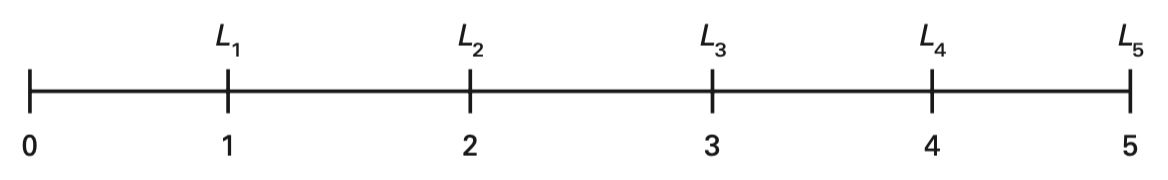
\includegraphics[scale=.5]{1}
\end{frame}

\begin{frame}{Processus d'appariement des flux de trésorerie}
\begin{block}{Étape 1}
Flux de trésorerie de l'obligation $A$ sélectionné pour satisfaire $L_5$
\begin{itemize}[label=\bullet]
\item Coupon$=A_s$ 
\item Principal $=A_p$
\item $A_s+A_p=L_5$
\end{itemize}
\end{block}
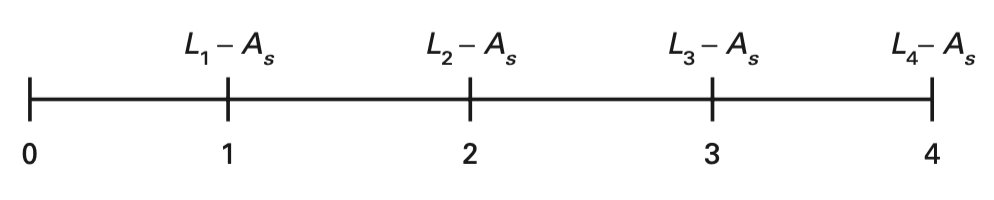
\includegraphics[scale=.5]{2}
\end{frame}

\begin{frame}{Processus d'appariement des flux de trésorerie}
\begin{block}{Étape 2}
Flux de trésorerie de l'obligation $B$ sélectionné pour satisfaire $L_4$
\begin{itemize}[label=\bullet]
\item Passif non provisionné = $L_4 - A_s$
\item Coupon$=B_s$ 
\item Principal $=B_p$
\item $B_s+B_p=L_4 - A_s$
\end{itemize}
\end{block}
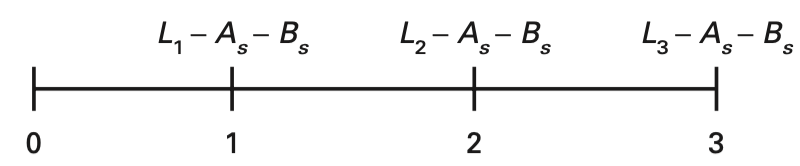
\includegraphics[scale=.5]{3}
\end{frame}


\begin{frame}{Processus d'appariement des flux de trésorerie}
\begin{block}{Étape 3}
Flux de trésorerie de l'obligation $C$ sélectionné pour satisfaire $L_3$
\begin{itemize}[label=\bullet]
\item Passif non provisionné = $L_3 - A_s-B_s$
\item Coupon$=C_s$ 
\item Principal $=C_p$
\item $C_s+C_p=L_3 - A_s-B_s$
\end{itemize}
\end{block}
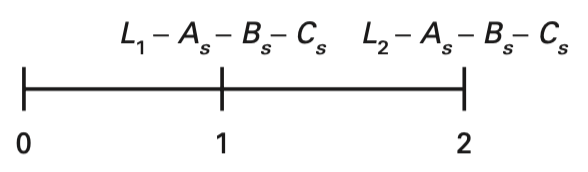
\includegraphics[scale=.5]{4}
\end{frame}

\begin{frame}{Processus d'appariement des flux de trésorerie}
\begin{block}{Étape 4}
Flux de trésorerie de l'obligation $D$ sélectionné pour satisfaire $L_2$
\begin{itemize}[label=\bullet]
\item Passif non provisionné = $L_2 - A_s-B_s-C_s$
\item Coupon$=D_s$ 
\item Principal $=D_p$
\item $D_s+D_p=L_3 - A_s-B_s-C_s$
\end{itemize}
\end{block}
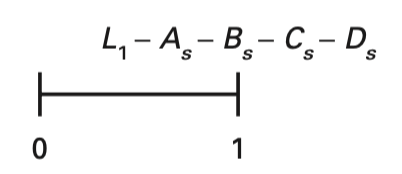
\includegraphics[scale=.5]{5}
\end{frame}

\begin{frame}{Processus d'appariement des flux de trésorerie}
\begin{block}{Étape 5}
Sélectionnez l'obligation E avec un flux de trésorerie de
\begin{align*}
 L_1 - A_s - B_s - C_s - D_s
\end{align*}
\end{block}

\end{frame}
\end{document}